\chapter{Исследовательский раздел}

В текущем разделе будет поставлена цель эксперимента, проведён сам эксперимент и сделаны соответствующие выводы.

\section{Технические характеристики}

Технические характеристики устройства, на котором выполнялось тестирование:

\begin{itemize}
	\item Операционная система: Ubuntu 20.04.3 \cite{ubuntu} Linux \cite{linux} x86\_64.
	\item Память: 8 GiB.
	\item Процессор: 11th Gen Intel® Core™ i5-1135G7 @ 2.40GHz \cite{intel};
	\item 4 физических ядра и 8 логических ядра.
\end{itemize}

Тестирование проводилось на ноутбуке, включенном в сеть электропитания. Во время тестирования ноутбук был нагружен только встроенными приложениями окружения, а также непосредственно системой тестирования.



\section{Постановка эксперимента}

\subsection{Цель эксперимента}

Цель эксперимента -- оценить зависимость времени работы от сложности запроса, поступающего на вход приложению.

\subsection{Время работы приложения}

Результаты замеров времени (в секундах) работы приложения приведены в таблице \ref{tbl:time}. Время посчитано как среднее арифметическое 100 замеров времени выполнения запросов. Перед каждым запросом в СУБД MySQL и PostgreSQL выполняется очистка кеша.

Запросы отдельно в СУБД MySQL и PostgreSQL выполнялись с выборкой из 1-5 столбцов. В листинге \ref{lst:time1} представлены запросы сразу с выборкой 5 стоблцов.

Также в листинге \ref{lst:time1} представлен запрос сразу в две СУБД одновременно, аналогично предыдущем, замеры выполнялись с выборкой 2-8 столбцов, запрос представлен сразу с выборкой 8 столбцов.


\begin{center}
	\captionsetup{justification=raggedright,singlelinecheck=off}
	\begin{lstlisting}[label=lst:time1,caption=Запросы для проведения эксперимента]
	-- Запрос в MySQL
	select t.tourid, t.nametour, t.typetour, t.countryid, t.duration
	from sys.tours as t
	
	-- Запрос в PostgreSQL 
	select h.hotelid , h.namehotel, h.countryid, h.region, h.categoryid
	from hotels as h
	
	-- Запрос сразу в две СУБД
	select t.tourid, t.nametour, t.typetour, t.duration, t.hotelid, t.travelonoff, t.powersupply, c.namecountry
	from db2.public.sys.tours as t join db1.postgres.public.countries as c on t.countryid = c.countryid
	\end{lstlisting}
\end{center}

Результаты замеров времени представлены в таблице \ref{tbl:time}.

На рисунке \ref{img:res1} представлены графики, основанные на результатах замеров времени выполнения запросов отдельно в СУБД и через приложения.

На рисунке \ref{img:res2} представлен график замеров времени выполнения запроса одновременно в две СУБД через приложение.


\begin{table}[!h]
	\begin{center}
		\captionsetup{justification=raggedleft,singlelinecheck=off}
		\caption{Результаты замеров времени (сек) работы приложения}
		\label{tbl:time}
		\begin{tabular}{|c|c|c|c|}
			\hline
			\multicolumn{4}{|c|} {MySQL} \\ \cline{1-4}
			\textbf{Запроc (кол-во столбцов)} & \textbf{Приложение} & \textbf{СУБД} & \textbf{Разница}\\
			\hline
			1 & 0.000652 & 0.000395 & 0.000257\\
			\hline
			2 & 0.000784 & 0.000485 & 0.000298\\
			\hline
			3 & 0.000815 & 0.000536 & 0.000278\\
			\hline
			4 & 0.000909 & 0.000658 & 0.000351\\
			\hline
			5 & 0.000998 & 0.000789 & 0.000209\\
			\hline
			\multicolumn{4}{|c|} {PostgreSQL} \\ \cline{1-4}
			\textbf{Запроc (кол-во столбцов)} & \textbf{Приложение} & \textbf{СУБД} & \textbf{Разница}\\
			\hline
			1 & 0.000721 & 0.000495 & 0.000225\\
			\hline
			2 & 0.000801 & 0.000575 & 0.000225\\
			\hline
			3 & 0.000858 & 0.000621 & 0.000237\\
			\hline
			4 & 0.000903 & 0.000721 & 0.000182\\
			\hline
			5 & 0.000989 & 0.000857 & 0.000132\\
			\hline
		\end{tabular}
	\end{center}
	
\end{table}

\begin{figure}[h!]
	\begin{center}
		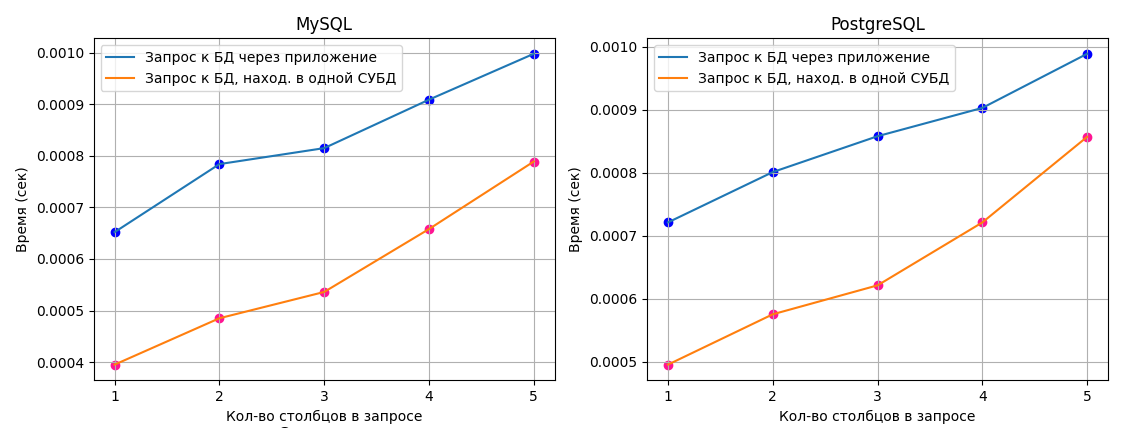
\includegraphics[scale=0.55]{./inc/img/res1}
		\caption{Графики, основанные на результатах замеров времени выполнения запросов отдельно в СУБД и через приложения}
		\label{img:res1}
	\end{center}
\end{figure}


\begin{figure}[h!]
	\begin{center}
		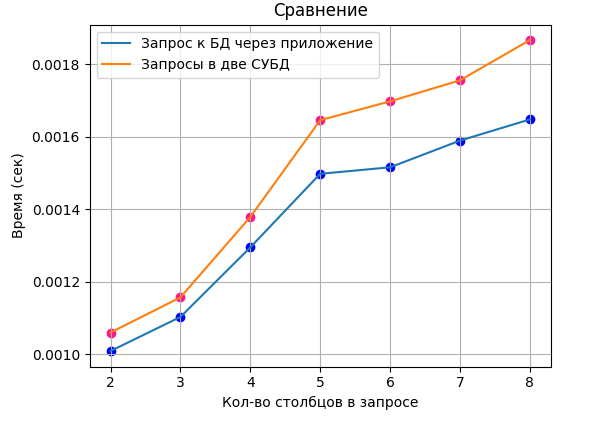
\includegraphics[scale=0.7]{./inc/img/res2}
		\caption{График замеров времени выполнения запроса одновременно в две СУБД через приложение}
		\label{img:res2}
	\end{center}
\end{figure}

\newpage

\section{Вывод}

В результате эксперимента было выявлено, что запросы через приложение работают медленнее, чем запросы сразу в СУБД в случае, если в запросах используются таблицы, которые расположены в одной конкретной СУБД, что видно на рисунке \ref{img:res1}. 

В случае, когда запрашиваются данные, находящиеся в двух различных СУБД, запрос, выполненный через приложение работает быстрее, чем запросы, выполняющиеся отдельно в каждую СУБД, что видно на рисунке \ref{img:res2}.
